\documentclass{article}

\usepackage{geometry}
\usepackage{amsmath}
\usepackage{graphicx, eso-pic}
\usepackage{listings}
\usepackage{hyperref}
\usepackage{multicol}
\usepackage{fancyhdr}
\pagestyle{fancy}
\fancyhf{}
\hypersetup{ colorlinks=true, linkcolor=black, filecolor=magenta, urlcolor=cyan}
\geometry{ a4paper, total={170mm,257mm}, top=40mm, right=20mm, bottom=20mm, left=20mm}
\setlength{\parindent}{0pt}
\setlength{\parskip}{0.3em}
\renewcommand{\headrulewidth}{0pt}
\rfoot{\thepage}
\lfoot{Seleksi IEEEXtreme 15.0 ITB}
\lstset{
    basicstyle=\ttfamily\small,
    columns=fixed,
    extendedchars=true,
    breaklines=true,
    tabsize=2,
    prebreak=\raisebox{0ex}[0ex][0ex]{\ensuremath{\hookleftarrow}},
    frame=none,
    showtabs=false,
    showspaces=false,
    showstringspaces=false,
    prebreak={},
    keywordstyle=\color[rgb]{0.627,0.126,0.941},
    commentstyle=\color[rgb]{0.133,0.545,0.133},
    stringstyle=\color[rgb]{01,0,0},
    captionpos=t,
    escapeinside={(\%}{\%)}
}

\begin{document}

\begin{center}
    \section*{Jebakan Penyihir} % ganti judul soal

    \begin{tabular}{ | c c | }
        \hline
        Batas Waktu  & 2 s \\    % jangan lupa ganti time limit
        Batas Memori & 256 MB \\  % jangan lupa ganti memory limit
        \hline
    \end{tabular}
\end{center}

\subsection*{Deskripsi}
Bambi sedang berusaha keluar dari jebakan penyihir!

Jebakan penyihir dapat digambarkan dengan \textit{grid} 2 dimensi dengan $N$ baris dan $M$ kolom. Baris di jebakan penyihir dinomori $1$ sampai $N$, sedangkan kolom di jebakan penyihir dinomori $1$ sampai $M$. Sel jebakan penyihir yang berada di baris ke-$r$ dari atas dan kolom ke-$c$ dari kiri dinyatakan dengan $(r, c)$. Setiap sel jebakan penyihir dapat berupa salah satu dari empat jenis sel berikut.
\begin{itemize}
    \item \verb|'.'|: jalan yang dapat dilewati Bambi
    \item \verb|'#'|: pagar yang tidak dapat dilewati Bambi
    \item \verb|'A'|: posisi Bambi saat ini
    \item \verb|'B'|: pintu keluar jebakan penyihir.
\end{itemize}

Untungnya, Bambi dapat bergerak dalam jebakan penyihir ini. Apabila Bambi berada di sel $(r,c)$, dalam satu langkah, Bambi dapat melakukan 8 jenis langkah berikut.
\begin{enumerate}
    \item bergerak ke $(r, c+1)$
    \item bergerak ke $(r+1, c+1)$
    \item bergerak ke $(r+1, c)$
    \item bergerak ke $(r+1, c-1)$
    \item bergerak ke $(r, c-1)$
    \item bergerak ke $(r-1, c-1)$
    \item bergerak ke $(r-1, c)$
    \item bergerak ke $(r-1, c+1)$
\end{enumerate}
Dengan kata lain, dalam satu langkah, Bambi dapat bergerak ke $8$ sel di sekitarnya. Selain itu, sel tujuan Bambi harus \textbf{berada dalam \textit{grid}} dan \textbf{bukan merupakan sel} \verb|'#'|.

Karena dikutuk oleh penyihir, Bambi memiliki batasan berikut dalam bergerak.
\begin{itemize}
    \item Setelah menggunakan langkah jenis $x$, Bambi harus menggunakan $3$ jenis langkah lain sebelum menggunakan langkah jenis $x$ lagi.
\end{itemize}
Hitunglah langkah minimum yang perlu dilakukan Bambi untuk bergerak dari sel \verb|'A'| ke sel \verb|'B'|, atau nyatakan bahwa Bambi tidak mungkin mencapai sel \verb|'B'|.

\subsection*{Format Masukan}
Baris pertama masukan berisi dua bilangan bulat positif $N$ dan $M$ $(4 \leq N \times M \leq 10^4)$. 

Masing-masing dari $N$ baris berikutnya berisi $M$ karakter yang menyatakan jenis sel di jebakan penyihir. Setiap karakter merupakan salah satu dari \verb|.|, \verb|#|, \verb|A|, dan \verb|B|. Dijamin karakter \verb|A| dan \verb|B| muncul tepat satu kali.


\subsection*{Format Keluaran}
Keluaran terdiri atas satu baris berisi satu bilangan. Apabila Bambi tidak mungkin mencapai sel \verb|'B'| dari sel \verb|'A'|, bilangan ini bernilai $-1$. Apabila sebaliknya, bilangan ini bernilai langkah minimum yang perlu dilakukan Bambi untuk bergerak dari sel \verb|'A'| ke sel \verb|'B'|.

\begin{multicols}{2}
\subsection*{Contoh Masukan 1}
\begin{lstlisting}
3 6
......
A....B
......
\end{lstlisting}
\columnbreak
\subsection*{Contoh Keluaran 1}
\begin{lstlisting}
6
\end{lstlisting}
\vfill
\null
\end{multicols}

\begin{multicols}{2}
\subsection*{Contoh Masukan 2}
\begin{lstlisting}
2 6
B....A
##.#.#
\end{lstlisting}
\columnbreak
\subsection*{Contoh Keluaran 2}
\begin{lstlisting}
7
\end{lstlisting}
\vfill
\null
\end{multicols}

\begin{multicols}{2}
\subsection*{Contoh Masukan 3}
\begin{lstlisting}
6 3
#A#
#.#
#.#
#.#
#.#
#B#
\end{lstlisting}
\columnbreak
\subsection*{Contoh Keluaran 3}
\begin{lstlisting}
-1
\end{lstlisting}
\vfill
\null
\end{multicols}

\subsection*{Penjelasan}
Salah satu perjalanan yang mungkin ditempuh Bambi pada contoh 1 adalah seperti berikut.
\begin{center}
    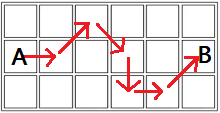
\includegraphics[]{grid-1.png}
\end{center}
Terlihat bahwa Bambi memerlukan $6$ langkah untuk bergerak dari sel \verb|'A'| ke sel \verb|'B'|. Bambi tidak mungkin mencapai sel \verb|'A'| ke sel \verb|'B'| dengan kurang dari $6$ langkah.
\end{document}